% !TEX TS-program = pdflatex
% !TEX encoding = UTF-8 Unicode
% !TEX root = main.tex
% !TEX spellcheck = en-US
% ****************************************************************************************
% File: thesis.tex
% Author: Patrick Haselwanter
% Date: 2023-10-28
% ****************************************************************************************
\documentclass[a4paper,11pt,oneside,final,titlepage,openany,onecolumn]{report}
% input preamble (include additional packages, set options, define macros)
% !TEX TS-program = pdflatex
% !TEX encoding = UTF-8 Unicode
% !TEX root = ../main.tex
% !TEX spellcheck = en-US
% ****************************************************************************************
% File: _preamble.tex
% Author: Patrick Haselwanter
% Date: 2023-10-28
% ****************************************************************************************

% ****************************************************************************************
% General settings (input encoding, font encoding, font, language)
% ****************************************************************************************
\usepackage[utf8]{inputenc} % character encoding used in input file
\usepackage[T1]{fontenc} % specifies the encoding used in the fonts
\usepackage{lmodern} % provides more support for non-ASCII characters than cm-super
\usepackage{microtype} % improves line-filling when using PDFLaTeX
\usepackage[ngerman,english]{babel} %  last language is considered the main one
\renewcommand{\familydefault}{\sfdefault} % select a sans serif font family 

\pdfsuppresswarningpagegroup=1 % suppress warning when including PDFs with page groups

% ****************************************************************************************
% Basic macros for thesis
% ****************************************************************************************
\newcommand{\authorAName}{Liam Nolan}
\newcommand{\authorAContact}{nl6496@mci4me.at}
\newcommand{\authorBName}{Johannes Schmid}
\newcommand{\authorBContact}{sj0751@mci4me.at}
\newcommand{\authorCName}{Jakob Spindler}
\newcommand{\authorContact}{sj0458@mci4me.at}
\newcommand{\courseName}{WS 2024 Computational Methods of Fluid Dynamics}
\newcommand{\courseCode}{MECH-M-3-CFD-NSM-VO}
\newcommand{\department}{Department of Technology \& Life Sciences}
\newcommand{\docTitle}{Optimization Study of a flow heater}
\newcommand{\docType}{Report}
\newcommand{\studyProgram}{Master's program Mechatronics \& Smart Technologies}
\newcommand{\studyYear}{MA-MECH-23-VZ}
\newcommand{\lecturerName}{Manuel Berger, PhD}
\newcommand{\lecturerContact}{manuel.berger@mci.edu}
\newcommand{\university}{Management Center Innsbruck}
% Definition of BibTeX macro used in IEEEexample
\newcommand{\BibTeX}{BibTeX}

% ****************************************************************************************
% Drawing and plotting, scientific packages, 
% ****************************************************************************************
% For use of subfigure environment
\usepackage{subcaption}

% For use of cmidrule in table environment
\usepackage{booktabs}

\usepackage{makecell}

% Handling of images
\usepackage{graphicx}
\graphicspath{{./img/}}

% Colour support
\usepackage[table]{xcolor}

% Handling of MATLAB code
\usepackage{mcode}

% Tabulars with adjustable-width columns
\usepackage{tabularx}
\usepackage{multirow}

% Sketching and importing MATLAB plots
\usepackage{pgfplots}
\usepackage{grffile}
\pgfplotsset{compat=newest}
\usetikzlibrary{plotmarks}
\usetikzlibrary{arrows.meta}
\usetikzlibrary{patterns}
\usepgfplotslibrary{patchplots}
\pgfplotsset{plot coordinates/math parser=false}
\newlength\figureheight
\newlength\figurewidth
\usepackage{svg}


% Typesetting electrical networks
\usepackage{circuitikz}

% scientific packages
\usepackage{amsmath}
\usepackage{amsfonts}
\usepackage{xfrac}
\usepackage{siunitx}
\AtBeginDocument{\sisetup{
	mode=match,
	unit-font-command = \mathrm,
	reset-text-family=false,
	reset-text-series=false,
	reset-text-shape=false,
	exponent-product=\cdot
}}
\DeclareSIUnit\unity{1} % can be used for dimensionless quantities
\DeclareSIUnit\sample{Sa}
% ****************************************************************************************
% Referencing and citing
% ****************************************************************************************
% Caption settings
\usepackage[
	format=plain, % typeset as normal paragraph
	labelformat=simple, % typeset label as name and number
	labelsep=period, % caption label and text separated by period and space
	textformat=simple, % caption text typeset as is
	justification=justified, % typset caption as normal paragraph
	singlelinecheck=true, % automatically center short captions
	font=small,
	labelfont=bf, % set bold font for label
	width=.75\textwidth % set fixed width for caption
]{caption}
\captionsetup[table]{position=top}
\captionsetup[figure]{position=bottom}

% Hypertext marks (should be loaded last but before geometry)
\usepackage[hyperindex]{hyperref}
% Extension options
\hypersetup{
	colorlinks, % colours the text of links and anchors (instead of borders)
	linkcolor={blue!65!black},
	citecolor={blue!65!black},
	urlcolor={blue!65!black}
}
% PDF display and information options
\hypersetup{
	pdftitle={\docTitle},
	pdfsubject={\docType},
	pdfauthor={},
	pdfkeywords={},
	pdfcreator={pdflatex},
	pdfproducer={LaTeX with hyperref}
}

% formatting of cross-references
\usepackage[capitalise]{cleveref}
\crefformat{equation}{(#2#1#3)}
\Crefformat{equation}{Equation~(#2#1#3)}

% ****************************************************************************************
% Bibliography settings
% ****************************************************************************************
% template from https://www.ieee.org/conferences/publishing/templates.html
%\bibliographystyle{IEEEtran} % choose the reference style


% ****************************************************************************************
% Glossary (acronyms, list of symbols) settings
% ****************************************************************************************
\usepackage[acronym,nomain,nonumberlist,nopostdot,sort=def,toc]{glossaries}
\renewcommand*{\glstextformat}[1]{\textcolor{black}{#1}} % make links appear black
\newglossary[slg]{symbolslist}{syi}{syg}{List of Symbols} % define custom glossary
\glsaddkey% define custom key
	{unit}% key
	{\glsentrytext{\glslabel}}% default value
	{\glsentryunit}% command analogous to \glsentrytext
	{\GLsentryunit}% command analogous to \Glsentrytext
	{\glsunit}% command analogous to \glstext
	{\Glsunit}% command analogous to \Glstext
	{\GLSunit}% command analogous to \GLStext
\glssetnoexpandfield{unit}
\makeglossaries % create makeindex files

\newglossarystyle{symbolsliststyle}{%
	\setglossarystyle{long3col}% style based on long3col
	\renewenvironment{theglossary}{%
		\begin{longtable}{lp{\glsdescwidth}>{\arraybackslash}p{2cm}}}%
		{\end{longtable}}%
	\renewcommand*{\glossaryheader}{% change the table header
		\bfseries Symbol & \bfseries Description & \bfseries Unit\\\hline%
		\endhead}%
	\renewcommand*{\glossentry}[2]{% change the displayed items
		\glstarget{##1}{\glossentryname{##1}}% name
		& \glossentrydesc{##1}% description
		& $\glsentryunit{##1}$% unit
		\tabularnewline
	}%
}

% ****************************************************************************************
% Page layout and headers
% ****************************************************************************************
% Specify page layout (paper name and orientation specified in document class options)
\usepackage[
	includeheadfoot, % includes the head of the page into total body
	ignoremp, % disregards marginal notes in determining the horizontal margins
	nomarginpar, % shrinks spaces for marginal notes to 0pt
	hmargin=1.5in, % left and right margin
	vmargin=1in, % top and bottom margin
	headheight=14pt %  height of header
]{geometry}

\usepackage{parskip} % helps in implementing paragraph layouts

% Header and footer settings
\usepackage{fancyhdr}
\pagestyle{fancy} % set page style to 'fancy'
\renewcommand{\chaptermark}[1]{\markboth{\thechapter.\ #1}{}}
% \renewcommand{\sectionmark}[1]{\markright{\thesection.\ #1}}
\fancyhf{} % clear all header and footer fields
\fancyhead[L]{\leftmark} % set left header location (chapter)
% \fancyhead[R]{\rightmark} % set right header location (section)
\fancyfoot[C]{\thepage} % set center footer location (page count)

% ****************************************************************************************
% Packages for testing purposes (can be deleted)
% ****************************************************************************************
\usepackage{lipsum}
\usepackage{blindtext}
\usepackage{todonotes}
% Matlab
\lstset{language=Matlab,%
    %basicstyle=\color{red},
    breaklines=true,%
    morekeywords={matlab2tikz},
    keywordstyle=\color{blue},%
    morekeywords=[2]{1}, keywordstyle=[2]{\color{black}},
    identifierstyle=\color{black},%
    stringstyle=\color{mylilas},
    commentstyle=\color{mygreen},%
    showstringspaces=false,%without this there will be a symbol in the places where there is a space
    numbers=left,%
    numberstyle={\tiny \color{black}},% size of the numbers
    numbersep=9pt, % this defines how far the numbers are from the text
    emph=[1]{for,end,break},emphstyle=[1]\color{red}, %some words to emphasise
    %emph=[2]{word1,word2}, emphstyle=[2]{style},    
}
% EOF
\loadglsentries{./tex/_defns.tex}
\begin{document}
	\pagenumbering{alph}
	% !TEX TS-program = pdflatex
% !TEX encoding = UTF-8 Unicode
% !TEX root = ../main.tex
% !TEX spellcheck = en-US
% ****************************************************************************************
% File: titlepage.tex
% Author: Patrick Haselwanter
% Date: 2023-10-28
% ****************************************************************************************

\thispagestyle{empty}
\pdfbookmark[0]{Title page}{titlepage} % sets a PDF bookmark
\thispdfpagelabel{} %  set page number shown in the tool bar of a PDF viewer
\begin{center}
	\textbf{\Huge \university}\par
	\vspace{8ex}\par
	\textbf{\LARGE \department}\par
	\vspace{4ex}\par
	\textbf{\Large \studyProgram}\par
	\vspace{4ex}\par
	
\includegraphics[scale = 0.75]{MCI_Logo.pdf}\par
	\vspace{4ex}\par
	\textbf{\LARGE \docType}\par
	\vspace{2ex}\par
	\textbf{composed as part of the course\\[0.5ex] \courseName{} (\courseCode)}\par
	\vspace{4ex}\par
	\textbf{about}\par
	\vspace{4ex}\par
	\textbf{\LARGE \docTitle}\par
	\vspace{4ex}\par
	\textbf{from}\par
	\vspace{4ex}\par
	\textbf{\Large \href{\authorAContact}{\authorAName}, \href{\authorBContact}{\authorBName} and \href{\authorContact}{\authorCName}}
\end{center}
\vspace{4ex}
\begin{tabular}{ll}
	Study program & \studyProgram\\[0.5ex]
	Year & \studyYear\\[0.5ex]
	Course & \courseName{} (\courseCode)\\[0.5ex]
   
	Name of lecturer & \href{\lecturerContact}{\lecturerName}\\[0.5ex]
	Submission deadline & February 14, 2024
\end{tabular}
\vfill
\begin{center}
	\today
\end{center}
%EOF
	\pagenumbering{Roman}
	\pdfbookmark[0]{\contentsname}{toc} % sets a PDF bookmark
	\tableofcontents
	\newcounter{romanpagecount}
	\setcounter{romanpagecount}{\value{page}}
	\clearpage
	\pagenumbering{arabic}
	% add content of thesis here
    
	% !TEX TS-program = pdflatex
% !TEX encoding = UTF-8 Unicode
% !TEX root = ../main.tex
% !TEX spellcheck = en-US
% ****************************************************************************************
% File: func_descr_and_theor_aspects.tex
% Author: Patrick Haselwanter, Christoph Ehrhardt
% Date: 2023-10-28
% ****************************************************************************************
\chapter{Meshing of the Domain}
\label{chapter:meshing}

\begin{figure}[htbp]
    \centering
    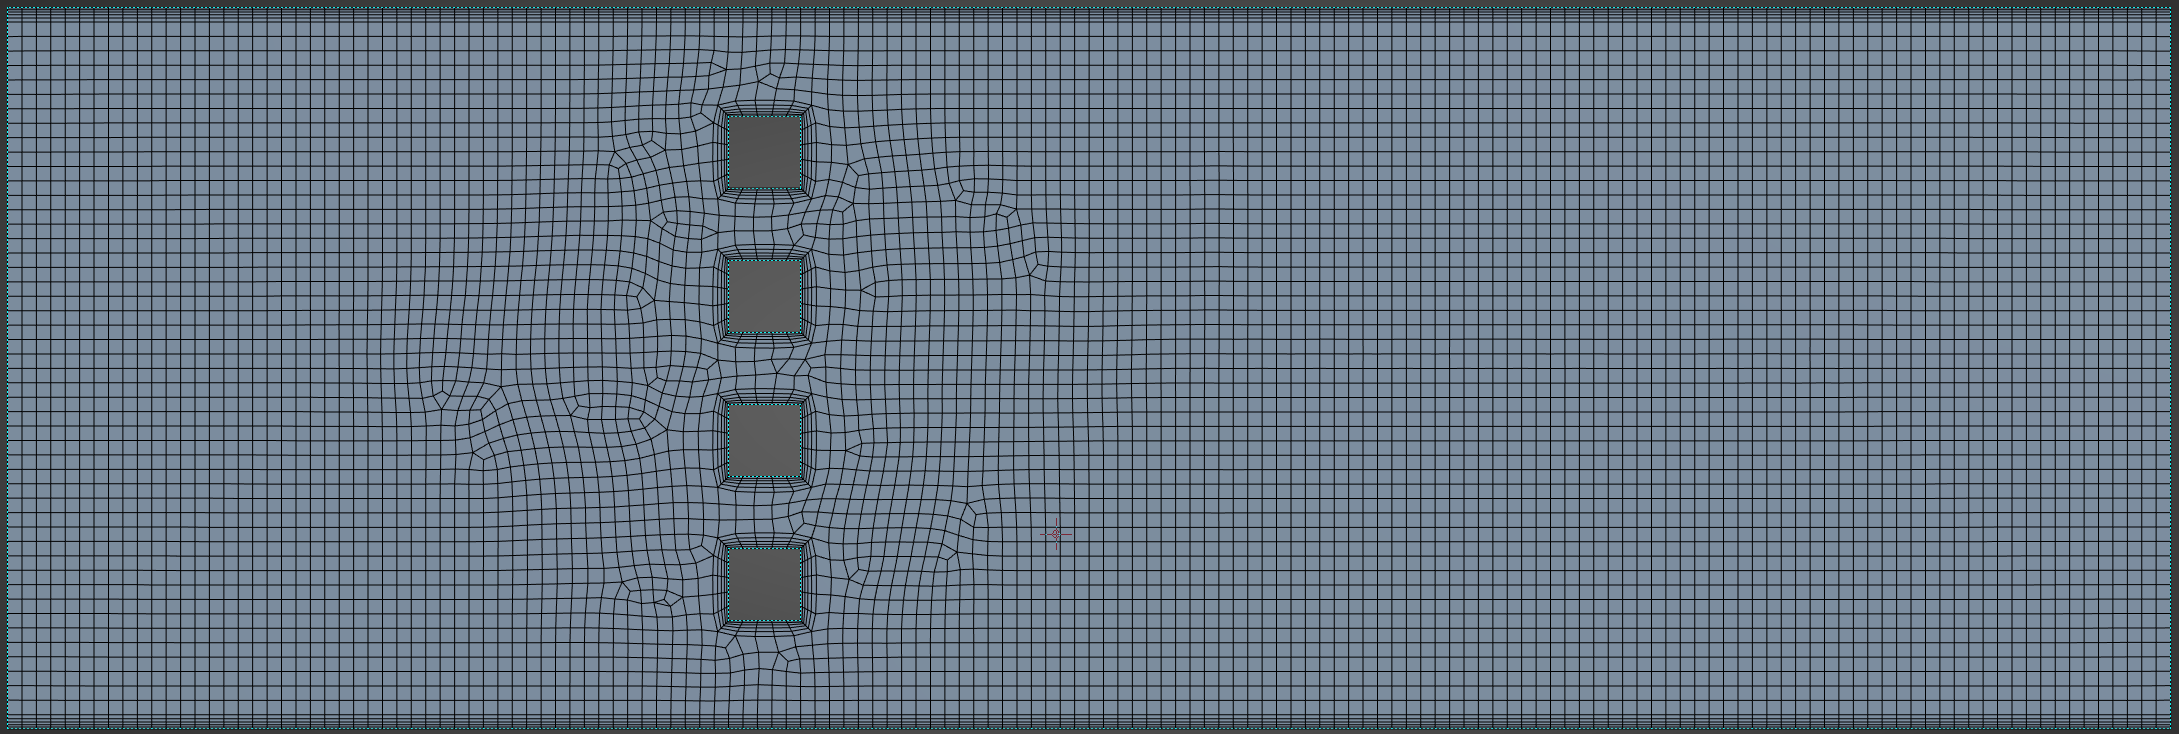
\includegraphics[width=0.8\textwidth]{img/meshing_base_geometry_full_view}
    \caption{Full view of the base geometry meshing}
    \label{fig:meshing_base_geometry_full_view}
\end{figure}


\begin{figure}[htbp]
    \centering
    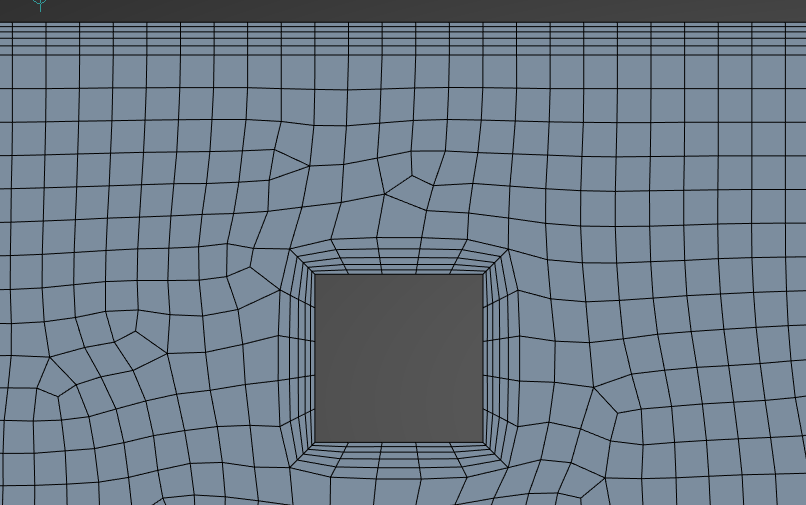
\includegraphics[width=0.8\textwidth]{img/meshing_base_geometry_detailed_view}
    \caption{Detailed view of the base geometry meshing}
    \label{fig:meshing_base_geometry_detailed_view}
\end{figure}


% EOF

	\chapter{Introduction}
\label{chap:Introduction}

This project focuses on the simulation of a steady-state 3D fluid flow and heat transfer problem within a flow heater, a configuration commonly found in process engineering applications. Accurately predicting both the flow field and temperature distribution is crucial to ensuring a homogeneous process environment, which directly impacts the overall quality of the process.

The geometry of the flow heater is shown in Figure \ref{fig:heater_geo}. For the purposes of this study, a 2D simplification (top-down view) was employed. This reduction in complexity allows for more efficient calculations and comparisons between different turbulence models, while maintaining a reasonable level of accuracy for the task at hand. The study primarily aimed to perform a Grid Convergence Study and evaluate various solver models, with results later applied to custom geometries for further simulations.

The flow heater in this case is examined under both laminar and turbulent flow conditions, leveraging different turbulence models to understand their effect on the heat transfer performance. The comparison of these models plays a key role in identifying the most appropriate solver configuration for real-world applications.

    \begin{figure}[h]   
    \centering
    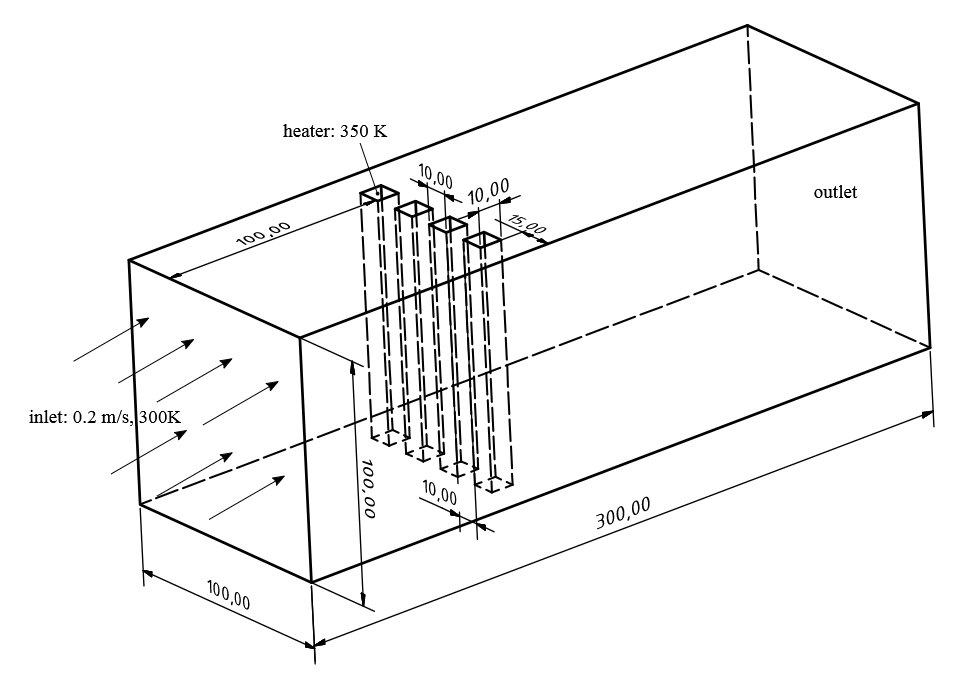
\includegraphics[width=0.65\textwidth]{img/heater_geo_og.png}
    \caption{Given heater geometry}
    \label{fig:heater_geo}
\end{figure}

% EOF

	\include{./tex/methods.tex}
	%% !TEX TS-program = pdflatex
% !TEX encoding = UTF-8 Unicode
% !TEX root = ../main.tex
% !TEX spellcheck = en-US
% ****************************************************************************************
% File: measurements.tex
% Author: Patrick Haselwanter
% Date: 2023-10-28
% ****************************************************************************************
\chapter{Hardware Implementation and Results}
\label{chapter:measurements}
\section{Hardware Implentation}
\label{sec:HI}
The setup of the real hardware is shown in \cref{fig:measurement_test_setup}.
\begin{figure}[htbp]
	\centering
	\includegraphics[width=0.5\textwidth]{img/setup.jpg}
	\caption{Real hardware setup}
	\label{fig:measurement_test_setup}
\end{figure}
It is composed of a cylinder in which a table tennis ball can move up and down. A fan mounted under the cylinder serves as the actuator that moves the table tennis ball. The position of the ball is read by a sensor mounted above the cylinder. 
The fan is controlled via a separate power supply module. This converts the input voltage of 5V into a corresponding PWM signal depending on the control setpoint. The control setpoint is defined via a controller implemented in Simulink, Simulink communicates with an I/O module from National Instruments (NI) and this passes the analog output to the power supply module. 
There is a similar setup for reading out the sensor, here the analog signal is forwarded to Simulink via the I/O module from NI. 

To apply the controller described in chapter \ref{chap:contr_des} to a real system, the Simulink-file shown in chapter \ref{chap:sim} is used as a basic setup. Instead of the identified system of the real plant, some interfaces to the real plant have to be introduced. This is done with the \textit{Analog Input} block, which builds the interface to the distance sensor and an \textit{Analog Output} block, which builds the interface to the fan motor. For the hardware of the laboratory at MCI VI, the drivers for the I/O Module \textit{National Instruments PCI 6221} have to be installed on the PC. 

To be able to do the system identification described in chapter \ref{sec:sys_ident}, an offset and a gain had to be applied to the response of the system. In order to be able to use the same controller as for the identified system, this offset of $d=0.77$ and gain of $k=1.81$ has to be introduced now to the real system. In the Simulink model, this has been done with simple \textit{gain} and \textit{bias} blocks. 

The following figure shows the Simulink system with the introduced gain and offset-blocks. Additionally, this figure shows the analog in- and output blocks, needed as an interface to the real hardware. 
\begin{figure}[!h]
\centering
    \begin{subfigure}{\textwidth}
      \centering
      \includegraphics[width=1\linewidth]{img/real_layer1.png}
      \caption[Top level servo controlled system]{Top level servo controlled system with interface to the real hardware and introduced offsets ad gains}
      \label{fig:simlayer1}
    \end{subfigure}
    \begin{subfigure}{\textwidth}
      \centering
      \includegraphics[width=.8\linewidth]{img/real_layer2.png}
      \caption{Linear system with observer}
      \label{fig:simlayer2}
    \end{subfigure}   
    \caption[Simulink model used for the real hardware implementation]{Simulink model used for the real hardware implementation}
    \label{fig:Simulink_sim_model}
\end{figure}
%%%%%%%%%%%%%%%%%%%%%%%%%%%%%%%%%%%%%%%%%%%%%%%%%%%%%%%%%%%%%%%%%%%%%%%%%%%%%%%%%%%%
\section{Results}
\label{res}
To verify if the implemented control structure described in the previous chapter works properly on the real system, several input trajectory signals were defined, which the system was supposed to follow. 
\\In the following figure \ref{fig:step}, the system is supposed to follow step signals. 
\begin{figure}[!h]
\centering
    \begin{subfigure}{.5\textwidth}
      \centering
      \includesvg[width=1\linewidth]{img/01.svg}
      \caption{Step-reference 1}
      \label{fig:01}
    \end{subfigure}%
    \begin{subfigure}{.5\textwidth}
      \centering
      \includesvg[width=1\linewidth]{img/02.svg}
      \caption{Step-reference 2}
      \label{fig:02}
    \end{subfigure}
    \caption{Response to step trajectory references}
    \label{fig:step}
\end{figure}

As it can be seen, the hardware follows the trajectory with a certain overshoot . Additionally, differently from the simulation, the real hardware oscillates quite a bit around the desired step-setpoint.   case. In this figure, the voltage represents to the distance measured by the sensor. Through the sensor characteristic, this voltage can be converted to a distance value. The voltage to ball-height conversion can be seen in the following figure \ref{fig:volt_dist}. 
\begin{figure}[!h]
        \centering
        \includesvg[width=0.5\linewidth]{polyfit_sens_data.svg}
        \caption[Sensor voltage to ball-height characteristic]{Sensor voltage to ball-height characteristic}
        \label{fig:volt_dist}
\end{figure}

It can be seen that sensor does not follow a linear relationship between voltage and height. In addition to this nonlinear sensor characteristic, also the introduced offsets and gains have to be taken into account, when the voltage values are transformed into ball-height values. 
This voltage to height conversion can be applied equally also for the results described subsequently.  
In the following figure \ref{fig:04} the response to a reference trajectory consisting of several steps is shown. 
\begin{figure}[!h]
        \centering
        \includesvg[width=0.5\linewidth]{img/04.svg}
        \caption{Response to a trajectory containing several steps}
        \label{fig:04}
\end{figure}
\\In this figure it can be seen, that the system tries to follow the reference trajectory. However, since the time between the single steps is quite short, the hardware is not able to follow the reference trajectory perfectly. Especially in the first step, the system is not able to follow the reference and has a high overshoot. 
In the following figure \ref{fig:sine} the response to sinusoidal reference inputs is shown.

\begin{figure}[!h]
\centering
    \begin{subfigure}{.5\textwidth}
      \centering
      \includesvg[width=1\linewidth]{img/03.svg}
      \caption{Sine-reference - low freq and low amp}
      \label{fig:06}
    \end{subfigure}%
    \begin{subfigure}{.5\textwidth}
      \centering
      \includesvg[width=1\linewidth]{img/05.svg}
      \caption{Sine-reference 2 - middle freq and high amp}
      \label{fig:06}
    \end{subfigure}
    \begin{subfigure}{.5\textwidth}
      \centering
      \includesvg[width=1\linewidth]{img/06.svg}
      \caption{Sine-reference 3 - high freq and high amp}
      \label{fig:06}
    \end{subfigure}    
    \caption{Response to sinusoidal trajectory references}
    \label{fig:sine}
\end{figure}
As it can be seen, the hardware is able to follow the sinusoidal reference trajectory at low frequencies. However, if the trajectory-frequency is too high, the system response is too slow to follow the trajectory. Additionally, in all three frequency examples it can be seen, that the system has problems to follow the trajectory in the startup. In all cases, this results in a relatively high overshoot.  
    \include{./tex/discussion.tex}
    
	\pagenumbering{Roman}
	\setcounter{page}{\value{romanpagecount}}
	\stepcounter{page}
	\bibliography{IEEEabrv,mybibfile} % point BibTEX at the .bib files
	\addcontentsline{toc}{chapter}{\bibname}
	\listoffigures
	\addcontentsline{toc}{chapter}{\listfigurename}
%	\listoftables
%	\addcontentsline{toc}{chapter}{\listtablename}
%	\clearpage
	\printglossary[type=acronym] % input files created by makeindex
	\printglossary[type=symbolslist,style=symbolsliststyle] % input files created by makeindex
	\appendix
	% !TEX TS-program = pdflatex
% !TEX encoding = UTF-8 Unicode
% !TEX root = ../main.tex
% !TEX spellcheck = en-US
% ****************************************************************************************
% File: appendix.tex
% Author: Patrick Haselwanter
% Date: 2023-10-28
% ****************************************************************************************
\chapter{MATLAB scripts}
\label{chapter:MATLAB_script}
As attachment, all Matlab live scripts and Simiulink files used in in the context of this laboratory are submitted as \textit{.mlx}-files and \textit{.slx}-files. Additionally, the following live scripts are also directly attached to this report in written format: 
    \begin{itemize}
        \item response\_fitting\_lab\_data.mlx
        \item aerodynamic\_state\_observer\_controller\_init.mlx
    \end{itemize}
% EOF
\end{document}
% EOF